\section{Introduction}\label{sec:introduction}

In the Western music canon, 
\emph{melody} is a defining characteristic of musical composition, 
and can even constitute the very identity of a piece of music within the collective consciousness. 
Because of the significance of melody to our music perception, 
the ability to automatically transcribe the melody notes present in an arbitrary recording 
could enable numerous applications in 
% performance??
interaction~\cite{ryynanen2008accompaniment}, 
education~\cite{droe2006music}, 
informatics~\cite{bainbridge1999towards}, 
retrieval~\cite{ghias1995query}, 
source separation~\cite{ewert2014score},
and generation~\cite{hawthorne2019enabling}.
Despite the potential benefits, 
reliable melody transcription remains an open challenge.

A closely-related problem that has received considerable attention from the MIR community is \emph{melody extraction}~\cite{goto1999real,goto2004real,salamon2014melody,rao2022melody}, where the goal is to estimate the time-varying, continuous \fnot{} trajectory of the melody in an audio mixture. 
In contrast, the goal of melody transcription is to output the \emph{notes} of the melody, where a note is defined by an onset time, a pitch, and an offset time. 
While \fnot{} trajectories are useful for several downstream tasks (e.g.,~query by humming) and more inclusive of music which does not use equal-tempered pitches, unlike notes, trajectories cannot be readily converted into formats like MIDI or scores which are more convenient for musicians.

\begin{figure}
    \centering
    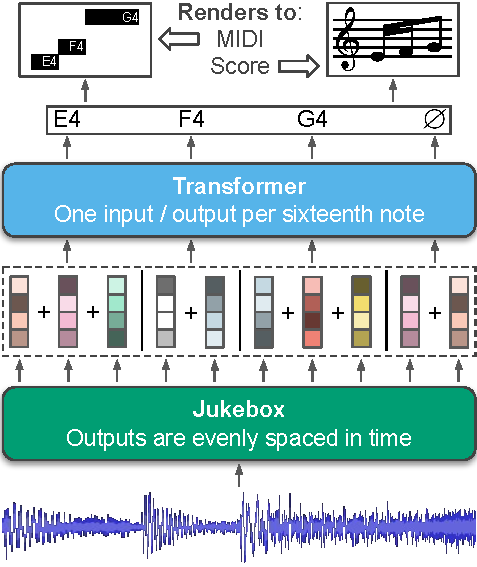
\includegraphics[width=8.1cm]{figs/fig1.pdf}
    \caption{
Our melody transcription approach involves 
(1)~extracting audio representations from Jukebox~\cite{dhariwal2020jukebox}, a generative model of music, 
(2)~averaging these representations across time to their nearest sixteenth note (dashed outline---uses \madmom{}~\cite{bock2016joint,bock2016madmom} for beat detection),
and
(3)~training a Transformer~\cite{vaswani2017attention} to detect note onsets (or absence thereof) per sixteenth note. 
Outputs can be rendered to MIDI (by mapping beats back to time) or a score.
}
 \label{fig:fig1}
 \vspace{-5mm}
\end{figure}

The relative lack of progress on melody transcription is perhaps counterintuitive when compared to the considerable progress on seemingly more difficult tasks like piano transcription~\cite{sigtia2016end,hawthorne2017onsets}.
%and chord recognition~\cite{humphrey2012rethinking,boulanger2013audio}. 
This circumstance stems from two primary factors.
First, unlike in piano transcription, melody transcription involves operating on \emph{broad}
audio mixtures from arbitrary instrument ensembles and musical styles. 
%Second, unlike in chord recognition, melody transcription involves isolating the notes from a single instrument voice (recognized to be the melodic voice) within the mixture. 
%Second, melody transcription involves not only detecting notes but also identifying which of those notes constitutes the melody, which may require modeling the nuances of human music perception. 
Second, there is a deficit of training data for melody transcription, which particularly impedes the deep learning approaches central to recent improvements on other transcription tasks. 
Moreover, collecting data for melody transcription is difficult compared to collecting data for tasks like piano transcription, where a Disklavier can be used to create aligned training data in real time. 

To overcome the challenge of transcribing broad audio, in this work we leverage representations from Jukebox~\cite{dhariwal2020jukebox}, a large-scale generative model of music audio pre-trained on $1$M songs. 
In~\cite{castellon2021calm}, Castellon~et~al.\ demonstrate that representations from Jukebox are useful for improving performance on a wide variety of MIR tasks. 
Here we show that, when used as input features to a Transformer model~\cite{vaswani2017attention}, representations from Jukebox yield 
% (RWC All) .744 vs .631 = 17.9%
% (Hookthr) .615 vs .514 = 19.6%
% (RWC Vox) .786 vs .621 = 26.6%
$27$\% stronger performance on melody transcription (as measured by note-wise F1) relative to handcrafted spectrogram features conventionally used for transcription. 
To our knowledge, this is the first evidence that representations learned via generative modeling are useful for time-varying MIR tasks like transcription, as opposed to the song-level tasks (e.g.~tagging, genre detection) examined in~\cite{castellon2021calm}.

To address the data deficit for melody transcription, 
we release a new dataset containing $50$ hours of melody annotations for broad audio 
which we derive 
from \hooktheory.\footnote{\url{https://www.hooktheory.com/theorytab}} 
The user-specified alignments between the audio and melody annotations in \hooktheory{} are crude---we refine these alignments using beat detection. 
To overcome remaining alignment jitter, we resample features to be uniformly spaced in beats (rather than time) and pass these \emph{beat-wise resampled} features as input to melody transcription models. 
This procedure 
has a secondary benefit of enabling simple conversion from raw model outputs to human-readable scores (\Cref{fig:fig1}).

By training Transformer models on this new dataset using representations from Jukebox as input, we are able to improve overall performance on melody transcription by 
% 0.786 vs 0.462 = 70%
% 0.744 vs 0.420 = 77%
$70$\% relative 
to the strongest available baseline. 
A summary of our primary \textbf{contributions} follows:
\begin{itemize}
    \item We show that representations from generative models can improve melody transcription (\Cref{sec:experiments}).
    \item We collect, align, and release a new dataset with $50$ hours of melody and chord annotations (\Cref{sec:dataset}).
    \item We propose a method for training transcription models on data with imprecise alignment (\Cref{sec:beatpool}).
    \item As a bonus application of our melody transcription approach, we build a system which can transcribe music audio into lead sheets (\Cref{sec:sheetsage}).
\end{itemize}